% Options for packages loaded elsewhere
\PassOptionsToPackage{unicode}{hyperref}
\PassOptionsToPackage{hyphens}{url}
\PassOptionsToPackage{dvipsnames,svgnames,x11names}{xcolor}
\documentclass[
  10pt,
  fontset=fandol]{ctexart}
\usepackage{xcolor}
\usepackage[margin=16mm]{geometry}
\usepackage{amsmath,amssymb}
\setcounter{secnumdepth}{-\maxdimen} % remove section numbering
\usepackage{iftex}
\ifPDFTeX
  \usepackage[T1]{fontenc}
  \usepackage[utf8]{inputenc}
  \usepackage{textcomp} % provide euro and other symbols
\else % if luatex or xetex
  \usepackage{unicode-math} % this also loads fontspec
  \defaultfontfeatures{Scale=MatchLowercase}
  \defaultfontfeatures[\rmfamily]{Ligatures=TeX,Scale=1}
\fi
\usepackage{lmodern}
\ifPDFTeX\else
  % xetex/luatex font selection
\fi
% Use upquote if available, for straight quotes in verbatim environments
\IfFileExists{upquote.sty}{\usepackage{upquote}}{}
\IfFileExists{microtype.sty}{% use microtype if available
  \usepackage[]{microtype}
  \UseMicrotypeSet[protrusion]{basicmath} % disable protrusion for tt fonts
}{}
\makeatletter
\@ifundefined{KOMAClassName}{% if non-KOMA class
  \IfFileExists{parskip.sty}{%
    \usepackage{parskip}
  }{% else
    \setlength{\parindent}{0pt}
    \setlength{\parskip}{6pt plus 2pt minus 1pt}}
}{% if KOMA class
  \KOMAoptions{parskip=half}}
\makeatother
\usepackage{graphicx}
\makeatletter
\newsavebox\pandoc@box
\newcommand*\pandocbounded[1]{% scales image to fit in text height/width
  \sbox\pandoc@box{#1}%
  \Gscale@div\@tempa{\textheight}{\dimexpr\ht\pandoc@box+\dp\pandoc@box\relax}%
  \Gscale@div\@tempb{\linewidth}{\wd\pandoc@box}%
  \ifdim\@tempb\p@<\@tempa\p@\let\@tempa\@tempb\fi% select the smaller of both
  \ifdim\@tempa\p@<\p@\scalebox{\@tempa}{\usebox\pandoc@box}%
  \else\usebox{\pandoc@box}%
  \fi%
}
% Set default figure placement to htbp
\def\fps@figure{htbp}
\makeatother
\setlength{\emergencystretch}{3em} % prevent overfull lines
\providecommand{\tightlist}{%
  \setlength{\itemsep}{0pt}\setlength{\parskip}{0pt}}
\usepackage{amsmath,amssymb,mathtools,needspace}
\xeCJKDeclareCharClass{CJK}{"2032,"0400->"04FF,"2160->"216B,"2460->"2473,"25A0,"25C7,"25CB,"25CF}
\IfFontExistsTF{Arial Unicode MS}{\xeCJKsetup{AutoFallBack=true}\setCJKfallbackfamilyfont{\CJKrmdefault}{Arial Unicode MS}}{}
\setcounter{secnumdepth}{0}
\setlength{\emergencystretch}{2em}
\allowdisplaybreaks
\usepackage{bookmark}
\IfFileExists{xurl.sty}{\usepackage{xurl}}{} % add URL line breaks if available
\urlstyle{same}
\hypersetup{
  pdftitle={Hadamard 阵的演化生成},
  colorlinks=true,
  linkcolor={Maroon},
  filecolor={Maroon},
  citecolor={Blue},
  urlcolor={Blue},
  pdfcreator={LaTeX via pandoc}}

\title{Hadamard 阵的演化生成}
\author{}
\date{}

\begin{document}
\maketitle

\subsubsection{10.3.4　Hadamard 阵的演化生成}\label{hadamard-ux9635ux7684ux6f14ux5316ux751fux6210}

上述镜像行复制的演化方式能否进一步简化呢？

从研究者的角度来说，平移对称比镜像对称更易于接受，而矩阵块比矩阵行更易于把握，现在进一步考察表 10.1 所列的平移块复制的演化方式。

考察某个方阵 \(A\)，直接对它施行平移正复制与平移反复制，分别生成 \([A\mathrel{\vdots}A]\) 与 \([A\mathrel{\vdots}-A]\)，两者合成在一起，得阶数倍增的方阵

\[
B=\begin{pmatrix}A&A\\A&-A\end{pmatrix}.
\]

这种演化方式称作\textbf{平移块复制}。

仍然从方波 \([+]\) 出发，反复施行平移块复制的演化方式，所生成的一系列方阵称作 \textbf{Hadamard 阵}。\(N\) 阶 Hadamard 阵记作 \(H_N\)。特别地，\(H_1=[+]\)。

显然，Hadamard 阵的演化机制同样从属于二分演化模式，如图 10.4 所示。

按平移块复制的演化方式，如果将 \(H_N\) 对分为 4 块，则其左上、右上与左下三块均为 \(H_{N/2}\)，而其右下则为 \(-H_{N/2}\)，即 Hadamard 阵有形式简单的递推表达式

\href{../../source-images/pdf-269.jpeg}{原页}

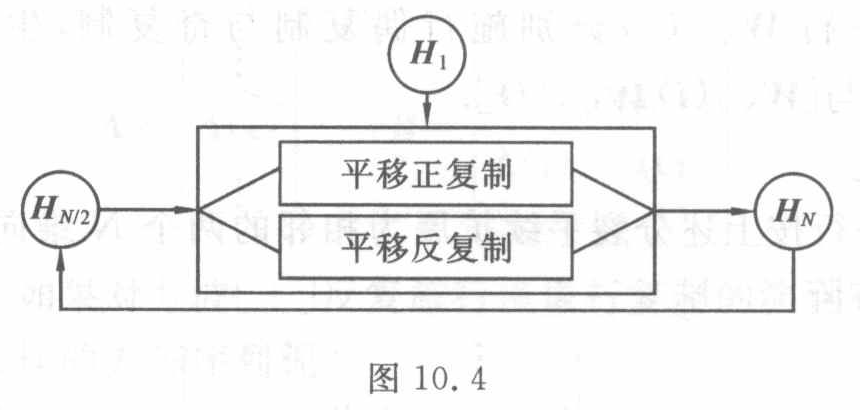
\includegraphics[width=0.85\linewidth,height=\textheight,keepaspectratio,alt={图 10.4（原图裁切）：Hadamard 阵的二分演化机制}]{../assets/ch10/fig-10-4.png}

图 10.4

\begin{quote}
图中文字与图意（转录）：初态 \(H_1\) 从上方进入；\(H_{N/2}\) 分成``平移正复制''和``平移反复制''两路，合成为 \(H_N\)；\(H_N\) 经下方反馈线返回 \(H_{N/2}\)。
\end{quote}

\[
H_N=\begin{pmatrix}H_{N/2}&H_{N/2}\\H_{N/2}&-H_{N/2}\end{pmatrix},\quad N=2,4,8,\cdots.
\tag{10.3.1}
\]

可见，Hadamard 阵的演化过程是简单的。事实上，从方波 \([+]\) 出发，按式（10.3.1）反复施行演化手续，有

\[
H_1=[+],
\]

\[
H_2=\begin{pmatrix}H_1&H_1\\H_1&-H_1\end{pmatrix}=\begin{pmatrix}+&+\\+&-\end{pmatrix},
\]

\[
H_4=\begin{pmatrix}H_2&H_2\\H_2&-H_2\end{pmatrix}=\begin{pmatrix}
+&+&+&+\\
+&-&+&-\\
+&+&-&-\\
+&-&-&+
\end{pmatrix},
\]

\[
H_8=\begin{pmatrix}H_4&H_4\\H_4&-H_4\end{pmatrix}=\begin{pmatrix}
+&+&+&+&+&+&+&+\\
+&-&+&-&+&-&+&-\\
+&+&-&-&+&+&-&-\\
+&-&-&+&+&-&-&+\\
+&+&+&+&-&-&-&-\\
+&-&+&-&-&+&-&+\\
+&+&-&-&-&-&+&+\\
+&-&-&+&-&+&+&-
\end{pmatrix}.
\]

如此继续下去，可以证明，这样演化生成的 Hadamard 阵同样是一种 Walsh 方阵。这里的 Hadamard 阵同 Walsh 阵相比较，两者只是行（列）的排序方式不同而已。

进一步考察矩阵元素的递推关系。前已指出，如果将矩阵 \(H_N\) 对分为 4 块，则其左上、右上与左下 3 块均为 \(H_{N/2}\)，而右下块则为 \(-H_{N/2}\)。记 \(H_N(i,j)\) 为矩阵 \(H_N\) 第 \(i\) 行第 \(j\) 列的元素，则上下两组\textbf{平移对} \((i,j)\)、\((i,N/2+j)\) 与 \((N/2+i,j)\)、\((N/2+i,N/2+j)\) 的矩阵元素有定理 10.1 所述的关系。

\textbf{定理 10.1}　对于 \(0\leqslant i,j\leqslant N/2-1\)，有

\[
\begin{aligned}
H_N(i,j)&=H_N(i,N/2+j)=H_N(N/2+i,j)\\
&=-H_N(N/2+i,N/2+j)=H_{N/2}(i,j).
\end{aligned}
\]

\href{../../source-images/pdf-270.jpeg}{原页}

现在基于 Hadamard 阵的上述表达式设计 Walsh 变换的快速算法 FWT。FWT 的设计同样从属于二分演化模式。

\begin{center}\rule{0.5\linewidth}{0.5pt}\end{center}

\subsection{相关原页校注（agent 补充）}\label{ux76f8ux5173ux539fux9875ux6821ux6ce8agent-ux8865ux5145}

以下校注来自本节覆盖的原页，可能也涉及同页相邻小节；原文照录与校正说明分开保留。

\subsubsection{原书 PDF 页 270 的校注}\label{ux539fux4e66-pdf-ux9875-270-ux7684ux6821ux6ce8}

\href{../pages/pdf-270.md}{完整原页转录} · \href{../../source-images/pdf-270.jpeg}{原页图像}

校注记录：CH10-E002。

\begin{quote}
校注（agent 补充，CH10-E002）：原文``对称正交阵''照录。依本章未归一化的 \(\pm1\) 元素定义，\(H_N^\mathsf{T}H_N=NI\)，\(N>1\) 时并非通常定义下满足 \(Q^\mathsf{T}Q=I\) 的正交矩阵；准确地说其行列两两正交，\(H_N/\sqrt N\) 才是正交矩阵。原页逆变换中的 \(1/N\) 因子与该定义一致。本项是原书术语疑误，不是 OCR 错误。
\end{quote}

\subsection{本节覆盖原页的校注记录}\label{ux672cux8282ux8986ux76d6ux539fux9875ux7684ux6821ux6ce8ux8bb0ux5f55}

下列记录按原页关联，含同页相邻小节的校注；计算时同时读取上文校注和完整原页。

\begin{itemize}
\tightlist
\item
  \texttt{CH10-E002}：原书 PDF 页 270
\end{itemize}

\end{document}
